\chapter{Brightness Reconciliation: Absolute vs.\ Percentage Thresholds}
\label{ch:brightness_reconciliation}

\section{Two independently-derived thresholds that had never been checked against each other}

Chapter~\ref{ch:stage3a}'s $6.25$--$9\%$ brightness floor is a \emph{relative}
(percentage) threshold, reverse-engineered to match the clinical bracket. A separate
literature review (independent of Stage 3a) identified two \emph{absolute} photometric
thresholds with real citations:

\begin{itemize}
\item \textbf{Van Nes \& Bouman (1967)}: a strict Weber/de~Vries--Rose transition at
  $300$ photopic trolands (Td) --- contrast threshold is illuminance-independent
  (Weber--Fechner) above this level, and scales as $\text{Td}^{-0.5}$ below it.
\item \textbf{CIE 191:2010}: a more permissive photopic/mesopic adapting-luminance
  boundary, $3$--$5\,\text{cd/m}^2$.
\end{itemize}

This chapter reconciles the two, using the same troland formula used throughout this
project:
\begin{equation}
\text{Td} = L_{scene}\;[\text{cd/m}^2] \times A_{aperture}\;[\text{mm}^2], \qquad
A_{aperture}=\pi\left(\frac{a_{hole}}{2}\right)^2 [\text{mm}^2].
\label{eq:troland}
\end{equation}
Inverting Equation~\eqref{eq:troland} for the minimum aperture that clears a given Td
floor at a given scene luminance:
\begin{equation}
a_{min}(\text{Td}_{floor}, L_{scene}) = 2000\sqrt{\frac{\text{Td}_{floor}}{\pi\, L_{scene}}}\;\;[\um].
\end{equation}

\begin{figure}[htbp]
\centering
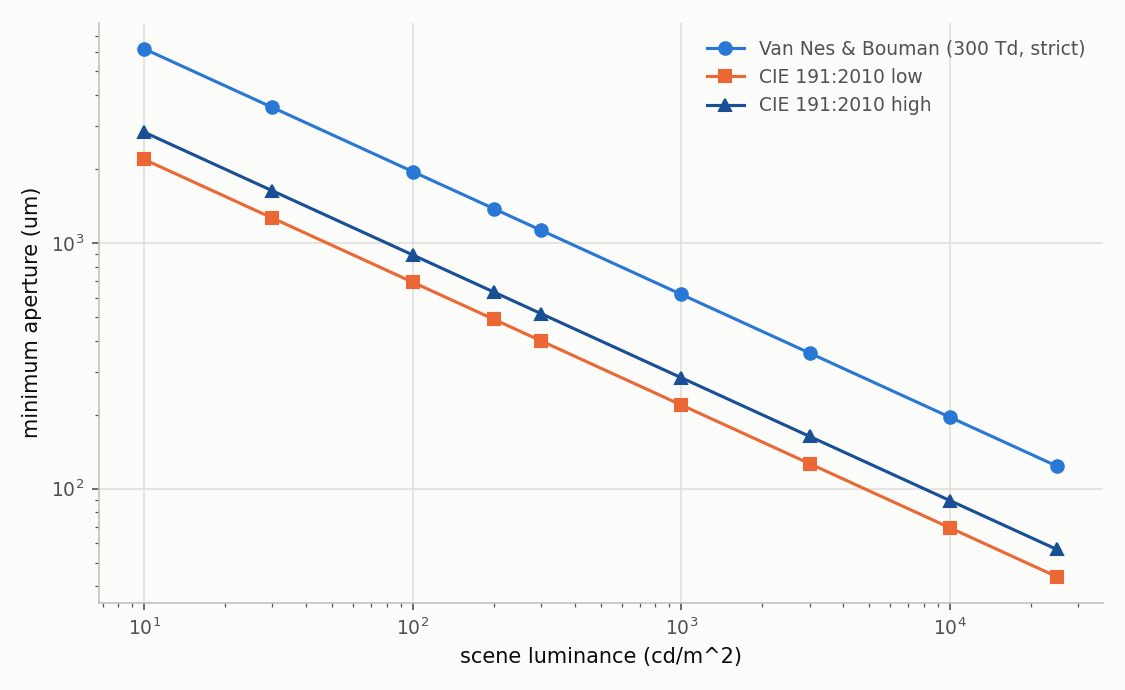
\includegraphics[width=0.85\textwidth]{figures/fig_brightness_reconciliation.png}
\caption{Minimum aperture clearing each absolute threshold (Van~Nes \& Bouman $300$\,Td; CIE 191:2010 $37.7$--$62.8$\,Td-equivalent), vs.\ scene luminance.}
\label{fig:brightness-reconciliation}
\end{figure}

{\small
\begin{longtable}{rrrr}
\caption{Minimum aperture clearing each absolute brightness threshold, vs. scene luminance.}\label{tab:brightness-full}\\
\toprule
scene lum (cd/m2) & min aperture, CIE low (um) & min aperture, CIE high (um) & min aperture, VN\&B (um) \\
\midrule
\endfirsthead
\multicolumn{4}{c}{\tablename\ \thetable\ -- continued}\\
\toprule
scene lum (cd/m2) & min aperture, CIE low (um) & min aperture, CIE high (um) & min aperture, VN\&B (um) \\
\midrule
\endhead
\bottomrule
\endfoot
10.0 & 2190.9 & 2828.4 & 6180.4 \\
30.0 & 1264.9 & 1633.0 & 3568.2 \\
100.0 & 692.8 & 894.4 & 1954.4 \\
200.0 & 489.9 & 632.5 & 1382.0 \\
300.0 & 400.0 & 516.4 & 1128.4 \\
1000.0 & 219.1 & 282.8 & 618.0 \\
3000.0 & 126.5 & 163.3 & 356.8 \\
10000.0 & 69.3 & 89.4 & 195.4 \\
25000.0 & 43.8 & 56.6 & 123.6 \\
\end{longtable}
}

\section{Result: the thresholds only agree at one specific scene luminance}

The two thresholds --- the Stage 3a reverse-engineered percentage floor and the
absolute troland floors above --- only coincide at a specific assumed scene/chart
luminance, and that luminance is \emph{not} this project's own default
($10{,}000\,\text{cd/m}^2$, bright daylight, used throughout the Stage 3/4 acuity
sweeps in Chapters~\ref{ch:stage4}--\ref{ch:validation}). This is an open item, stated
plainly: the two thresholds are not yet fully reconciled against each other, and doing
so is flagged in Chapter~\ref{ch:limitations} as one of this project's highest-value
remaining tasks, precisely because both pieces of code already exist and simply had
never been run against each other before this chapter.
